% Dokumentklassen:
% article, report, beamer, book, letter etc.
% https://en.wikibooks.org/wiki/LaTeX/Document_Structure
\documentclass[a4paper]{article}

% Seitenränder Abstand setzen
\usepackage[margin=80pt]{geometry}

% Deutsches Sprachpaket
\usepackage[ngerman]{babel}
% UTF8 Input Encoding
\usepackage[utf8]{inputenc}

% Schriftbild ändern
% https://en.wikibooks.org/wiki/LaTeX/Fonts
\usepackage[scaled]{helvet}
% (Sans) Serifen oder anderes
% \rmdefault: Serifen
% \sfdefault: Sans-Serifen
% \ttdefault: Typewriter
%\renewcommand{\familydefault}{\sfdefault}
% Fontencoding (für ä, ö, ü etc.)
\usepackage[T1]{fontenc}

% Gänsefüsschen richtig kompilieren
\usepackage [autostyle]{csquotes}
\MakeOuterQuote{"}

% Hyperlinks farblos
\usepackage[hidelinks]{hyperref}
\hypersetup{colorlinks=false}

% Package für Aufzählungen
\usepackage{enumitem}
% kein Abstand zwischen Aufzählungen
% Sollen doch Abstände vorhanden sein: nach Aufzählung {itemsep=1em}
\setlist{nosep}

% Grafik-Packages, für Figures, Subfigures und PDF als Import
\usepackage{graphicx}
\usepackage{subcaption}
\usepackage{pdfpages}

% Package und Einstellungen für Java-Code-Darstellung
% Werden erstellt mit \begin{lstlisting}
\usepackage{listings}
\usepackage{color}
\definecolor{dkgreen}{rgb}{0,0.6,0}
\definecolor{gray}{rgb}{0.5,0.5,0.5}
\definecolor{mauve}{rgb}{0.58,0,0.82}
\lstset{frame=tb,
	language=Java,
	aboveskip=3mm,
	belowskip=3mm,
	showstringspaces=false,
	columns=flexible,
	basicstyle={\small\ttfamily},
	numbers=none,
	numberstyle=\tiny\color{gray},
	keywordstyle=\color{blue},
	commentstyle=\color{dkgreen},
	stringstyle=\color{mauve},
	breaklines=true,
	breakatwhitespace=true,
	tabsize=3
}

\title{\textbf{Zusammenfassung MOBLAB} \\
		Mobile Programming Lab}
\date{\today}
\author{Maurin D. Thalmann}

\begin{document}
	
	\pagenumbering{gobble}
	\maketitle
	
	\newpage
	\pagenumbering{arabic}
	\tableofcontents
	
	\newpage
	
	\section{Tech-Intro}
	
		\subsection{Mobile Craftmanship Mindset}
		
		$\rightarrow$ \textbf{1:1 Portierung von Desktop zu Mobile reicht nicht aus!}
	
		\begin{itemize}
			\item Andere Benutzereingaben möglich auf Mobile: Touch, Pinch, Drag etc.
			\item Integrierte Sensoren: GPS, Kamera, Gyro, NFC, Bluetooth etc.
			\item Neue Einsatzmöglichkeiten: kontaktlose Interaktion, location-based, augmented etc.
		\end{itemize}
	
		\vspace{1em}
		
		\begin{itemize}
			\item Mindset der Entwickler \& Designer an neue Möglichkeiten anpassen
			\item Anforderungen \& Wünsche der Nutzer und des Markts prüfen (User-Interaction, Plattformstandards)
			\item Gute Entwickler kennen Plattformen, Betriebssysteme \& Bibliotheken
		\end{itemize}
	
		\subsection{Entwicklung mobiler Apps}
		
		\begin{figure}[htb!]
			\centering
			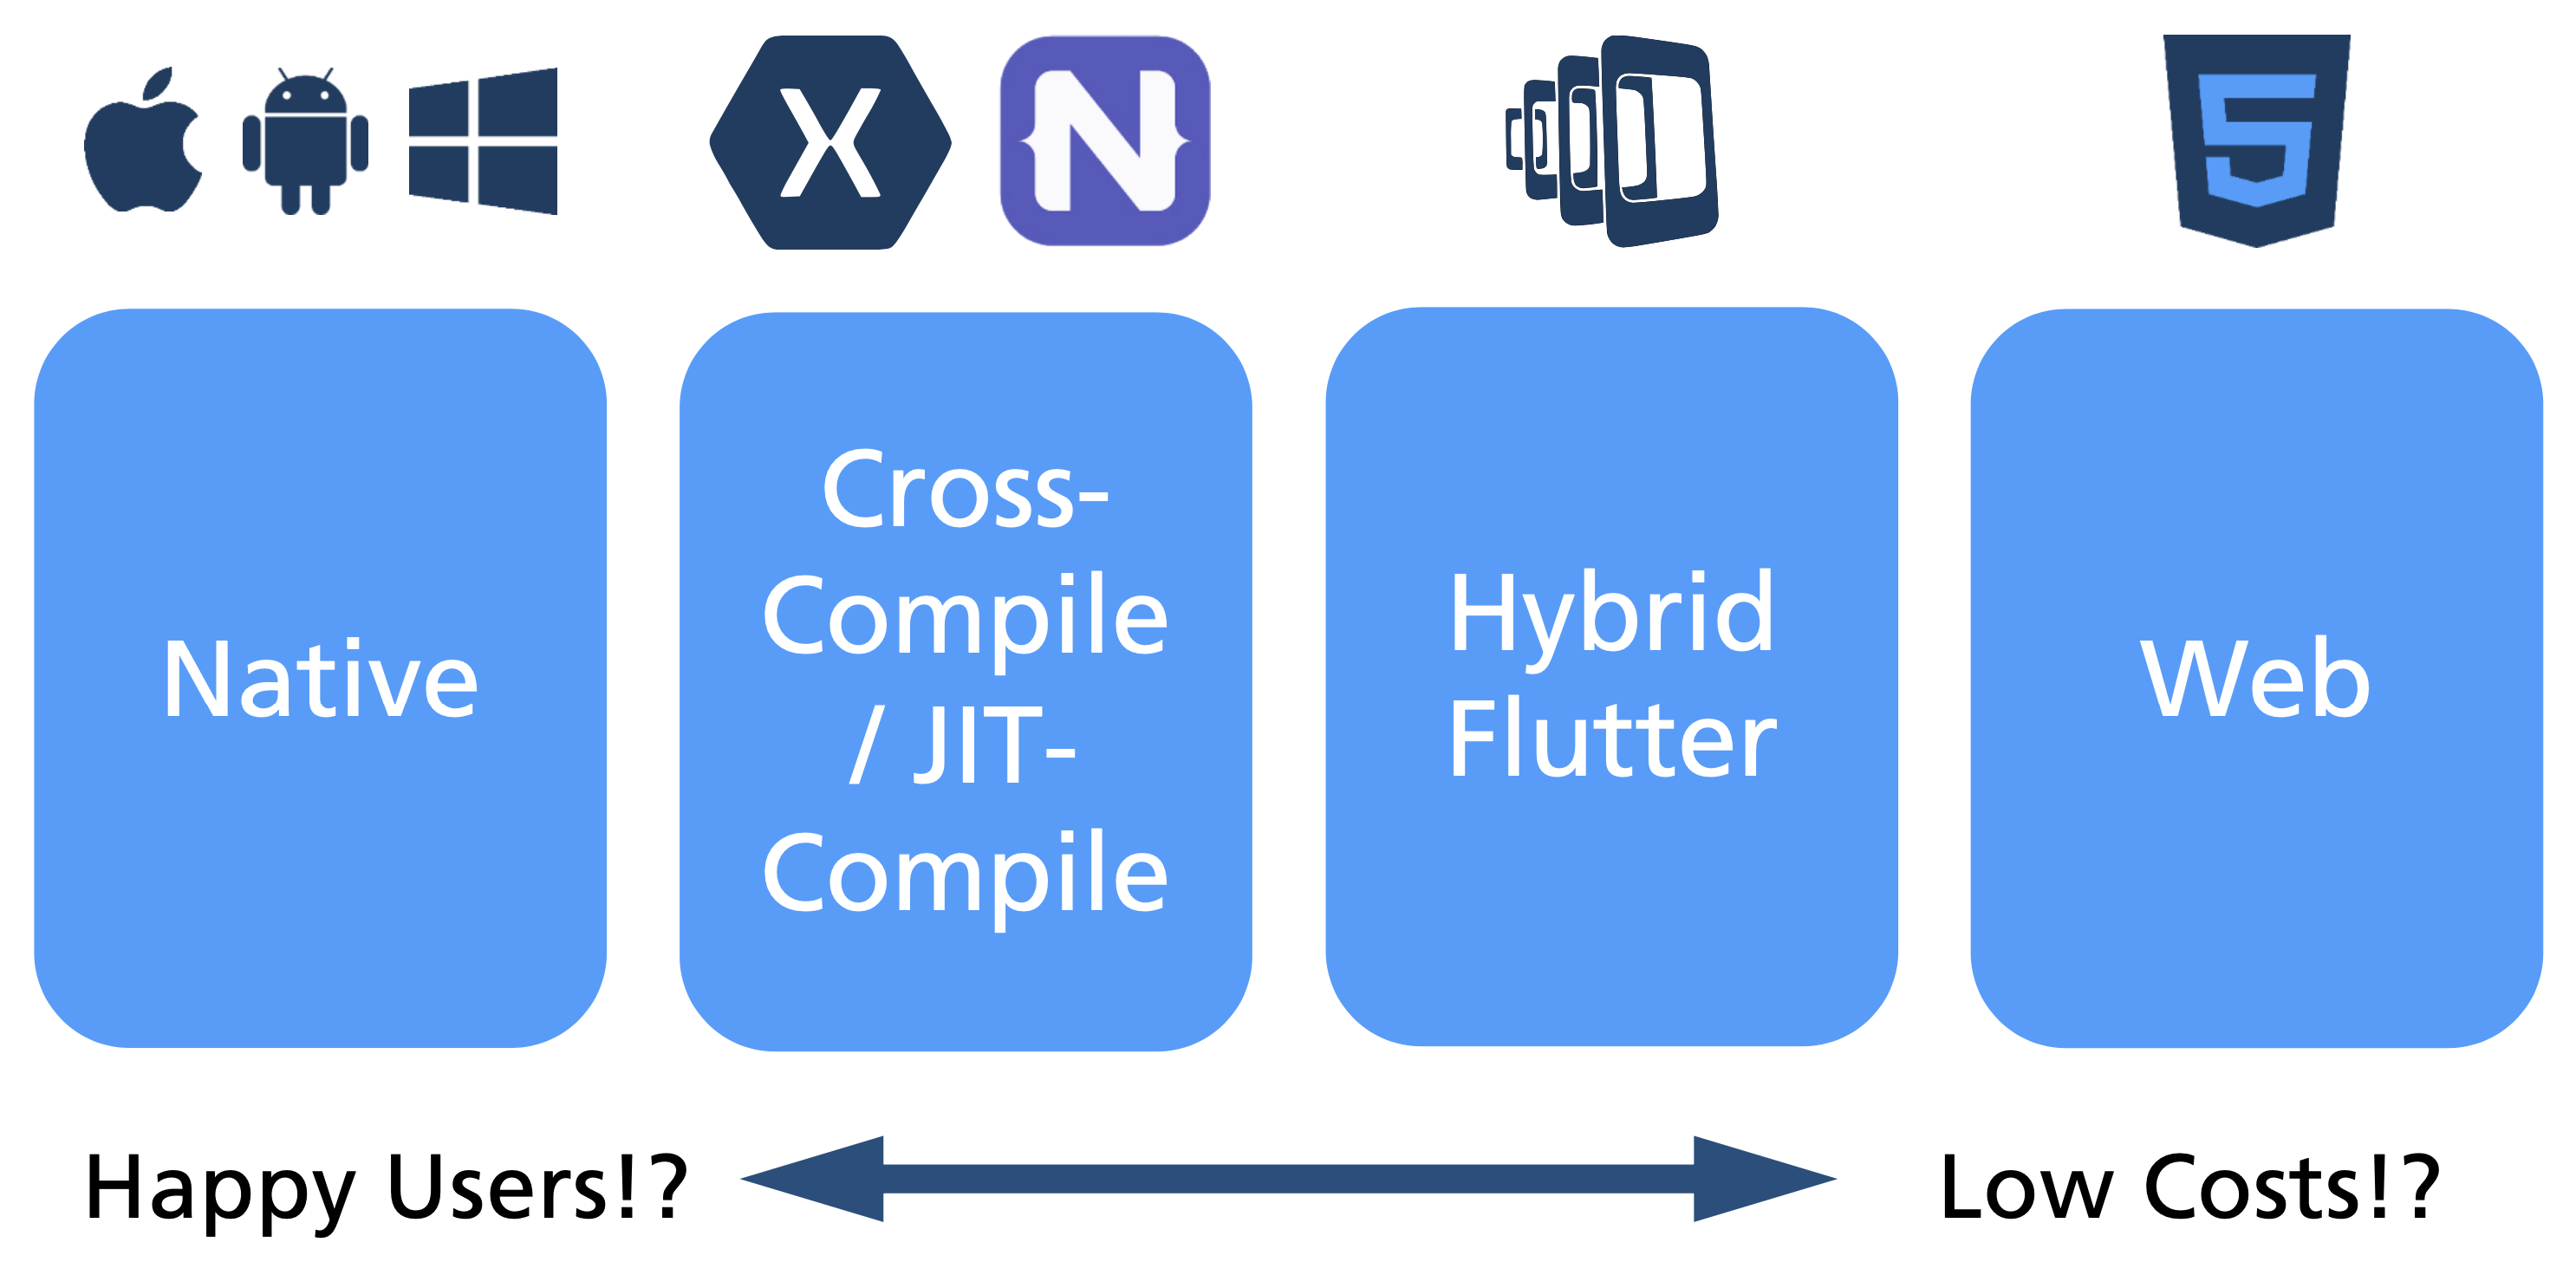
\includegraphics[width=0.7\textwidth]{img/techintro/spannungsfeld_apps.png}
			\caption{Das Spannungsfeld mobiler Entwicklung}
			\label{fig:techintro_spannungsfeld_apps}
		\end{figure}
	
		\begin{description}
			\item[Web-App] JS, HTML, CSS mit Responsive Design, im Browser ausgeführt
			\item[Hybrid] Web-App in nativem Wrapper verpackt, mit Connector-Plugins, kann als native App installiert werden (Cordova, Flutter etc.)
		\end{description}
		
	\section{SA - Kotlin \& Android}
	
	
	
	\section{SA - Data Binding \& ViewModel}
	
	
	
	\section{SA - Fastlane}
	
	
	
	\section{SA - Unreal Engine}
	
	
	
	\section{SA - Xamarin.Forms}
	
	
	
	\section{SA - PWA: Progressive Web Apps}
	
\end{document}
